% LAST UPDATED FOR 2019 SPRING GROUP MEETING

\documentclass{beamer}
\usecolortheme[RGB={109,121,147}]{structure}
\usetheme{Boadilla}
\setbeamercovered{invisible}

\setbeamertemplate{frametitle continuation}{}

\usepackage{amsmath}
\usepackage{booktabs}
\usepackage[T1]{fontenc}
\usepackage{graphicx}
\usepackage[round]{natbib}
\usepackage{lmodern}
\usepackage{tikz}
\usetikzlibrary{calc}
\usepackage{xcolor}
\definecolor{color0}{HTML}{8A94A9}
\colorlet{l-color0}{color0!50}

\newcommand{\EE}{\mathbb{E}}
\newcommand{\FF}{\mathcal{F}}
\newcommand{\PP}{\mathbb{P}}
\newcommand{\RR}{\mathbb{R}}
\newcommand{\ZZ}{\mathbb{Z}}
\newcommand{\cH}{\mathcal{H}}
\DeclareMathOperator*{\argmax}{arg\,max}
\DeclareMathOperator*{\se}{se}
\DeclareMathOperator{\sgn}{sign}

\newcommand{\hdelta}{\hat{\delta}}
\newcommand{\hmu}{\hat{\mu}}
\newcommand{\hsigma}{\hat{\sigma}}
\newcommand{\htheta}{\hat{\theta}}
\newcommand{\ao}{\alpha_0}
\newcommand{\gest}{\ge_\text{st}}
\newcommand{\vs}{\vskip+1em}

\graphicspath{{./fig/}}

\AtBeginSection[]{
  \begin{frame}
    \frametitle{Table of Contents}
    \tableofcontents[currentsection]
  \end{frame}
}

\title[Replicability Assessment]{Statistical Methods for Replicability Assessment}

\author[Hung \& Fithian]{Kenneth Hung and Will Fithian}
\institute[UC Berkeley]{
	University of California, Berkeley \\
	\medskip
	\textit{\{kenhung, wfithian\}@berkeley.edu}
}
\date{March 12, 2019}

\begin{document}

\begin{frame}
	\titlepage
\end{frame}

\iffalse
\begin{frame}
  \frametitle{First Author}
  \begin{center}
    \includegraphics[width=.5\textwidth]{kenneth-github.jpeg}\\
    Kenneth Hung (UC Berkeley Math)
  \end{center}
\end{frame}
\fi

\section{Reproducibility Project: Psychology}

\begin{frame}{Introduction: Replicability Crisis}
   \centering
   \includegraphics[width=0.8\textwidth]{nyt-title.png}
   \vs
   \includegraphics[width=0.8\textwidth]{nyt-body.png}
\end{frame}

\begin{frame}{Introduction: Replicability crisis}
  Social psychology facing urgent crisis in replicability of results
  % Oral: "Facing" as active verb: other fields have problems but they aren't facing it the way psych is
  \vs
  Commonly attributed to varied factors
  \begin{itemize}
	  \item selection for significance
	  \item $p$-hacking, questionable research practices (QRPs)
	  \item fraud
	  \item infidelity of replication experimental designs
	  \item flaws in original experimental designs
	  \item ``Hidden moderators'': subtle, uncontrollable differences in experimental conditions
  \end{itemize}
  % Oral: It makes quite a difference which of these is to blame, as I'll explain
  \vs
  Reproducibility Project:\ Psychology
  \begin{itemize}
	  \item Preregistered replications of $100$ studies published in 2008 in three top psych.\ journals
	  \item Massive collaborative effort by hundreds of researchers
  \end{itemize}
\end{frame}

\begin{frame}{Results from RP:P}
  RP:P reported descriptive statistics:
  \begin{itemize}
	  \item $36\%$ of replications significant in same direction as original study
	  \item $47\%$ of original point estimates in replication studies' $95\%$ CIs
	  \item $83\%$ of the effect size estimates declined ($\htheta_{i,R}/\htheta_{i,O} < 1$)
  \end{itemize}
  \vs 
  Widely reported as damning result:
  \begin{itemize}
	  \item {\em Washington Post}: ``... affirms that the skepticism [of published results] was warranted'' \citep{Achenbach:2015vi}
	  \item {\em Economist}: ``... managed to replicate satisfactorily the results
	    of only $39\%$ of the studies investigated'' \citep{Anonymous:uoQKTVTm}
	  \item {\em New York Times}: ``more than half of the findings did not hold up when retested'' \citep{Carey:2015wp}
  \end{itemize}
\end{frame}

\begin{frame}{Debate}
  What should we make of these numbers?
  \begin{itemize}
  	\item e.g.\ $47\%$ of original point estimates in replication studies' $95\%$ CIs 
  \end{itemize}
  \vs
  \citet{Gilbert:2016he} critiqued $47\%$ number:
  \begin{itemize}
	  \item Confidence interval $\ne$ predictive interval
	  \item No replication is exact ($\theta_{i,O} \ne \theta_{i,R}$)
	  \item Low fidelity of some replications (e.g.\ race questionnaire in Italy)
	  \item ``OSC seriously underestimated the reproducibility of psychological science''
  % Oral: not really fair in the sense that OSC didn't really estimate anything!
  \end{itemize}
  \vs
  Further debate between defenders \citep{Anderson:2016gs,Srivastava:2016,Nosek:2016}, critics \citep{Gilbert:2016uv,Gilbert:2016th}
\end{frame}

\begin{frame}{What estimand?}
  Did OSC ``underestimate replicability?''
  \vs
  First need to answer: what is the estimand?
  \vs
  RP:P offers
  \begin{itemize}
  	\item descriptive statistics
  	\item tiny $p$-values for tests of very strong nulls 
    \begin{itemize}
    	\item e.g.\ McNemar's test of whether orig.\ studies more likely to be significant at level $0.05$
    \end{itemize}
  	\item no attempt to define target of inference
  	\item no attempt to disentangle sources of error
  \end{itemize}
\end{frame}

\begin{frame}{Selection for significance}
  \centering
  RP:P data: unmistakable sign of selection at $\alpha = 0.05$

  \includegraphics[width=0.8\textwidth]{ecdf.pdf}

  {\color{red} Can this alone explain all results?}
\end{frame}

\begin{frame}{Simulation: Selection bias}
  Can selection bias alone explain RP:P's descriptive statistics?
  \vs
  Simulation experiment
  \begin{itemize}
  \item all original / replication studies: same effect size $\theta$
  \item Gaussian estimators $\htheta_{i,O}, \htheta_{i,R}$, $\text{s.e.} = 1$
  \item observe pair only when $|\htheta_{i,O}| > z_{\alpha/2}$
  \end{itemize}
  \vs
  Plot descriptive statistics as function of $\theta$
\end{frame}

\begin{frame}{Simulation: Selection bias}
  \centering
  {\bf Question:} with $\theta = 1/2$, what fraction of repl.\ CIs cover orig.\ estimates?
  \vs
  \pause
  \includegraphics[width=0.5\textwidth]{naive-ci-theta05.pdf}
  \vs
  {\bf Answer:} $\approx 50\%$
\end{frame}

\begin{frame}{Simulation: Selection bias}
  \centering
  \includegraphics[width=0.8\textwidth]{naive-ci-sim.pdf}
\end{frame}

\begin{frame}{Simulation: Selection bias}
  \centering
  \includegraphics[width=0.8\textwidth]{naive-same-dir.pdf}
\end{frame}

\begin{frame}{Simulation: Selection bias}
  \centering
  \includegraphics[width=0.8\textwidth]{naive-decline.pdf}
\end{frame}

\begin{frame}{Selection bias}
 
  Selection bias is basic feature of data
  \begin{itemize}
  \item Qualitatively, can explain RP:P metrics
  \item Can't learn anything else from data unless we adjust for it
  \end{itemize}
  \vs
  Different explanations suggest different priorities for reform, e.g.:
  \begin{itemize}
  \item Selection bias: publish negative results, post-hoc stat.\ adjustment
  \item Infidelities: more detailed methods sections?
  \item Hidden moderators: abandon experimental psychology?
  \end{itemize}
  \vs
  Key tools:
  \begin{itemize}
  \item conditional post-selection inference \citep[][many others]{Lee:2016fv, Fithian:2014ws}
  \item ideas from multiple testing \citep[][many others]{Benjamini:1995cd,Storey:2002vj,Heller:2007}
  \end{itemize}
\end{frame}

\section{Formalizing replicability}

\begin{frame}{A model for replications}
  Model for original (O) / replication (R) study pair $i = 1, \ldots, m$:
  \begin{equation}
  	\htheta_{i,O} \sim N\left(\theta_{i,O}, \;\sigma_{i,O}^2\right) 1_{\{|\htheta_{i,O}| > c\}} \quad\text{ and }\quad \htheta_{i,R} \sim N\left(\theta_{i,R}, \;\sigma_{i,R}^2\right)
  \label{eq:model}
  \end{equation}
  Can formalize three definitions in terms of parameters of model \eqref{eq:model}
  \begin{itemize}
  	\item Some hypotheses defined in terms of $S_i = \sgn(\htheta_{i,O})$
  \end{itemize}
  \vs
  Finite population model:
  \begin{itemize}
  	\item no assumptions on dist.\ of $(\theta_{i,O}, \theta_{i,R})$ 
  	\item agnostic to why $\theta_{i,O} \ne \theta_{i,R}$ 
  \end{itemize}
\end{frame}

\begin{frame}{Defining replicability}
  What do we estimate when we ``estimate replicability?''
  \vs
  {\bf RP:P statistic 1:} $36\%$ of replications significant in same direction as original study
  \vs
  {\bf Definition 1:} False directional claims
  \begin{itemize}
	  \item {\em What fraction of original directional claims were wrong?}
	  \item Psychology as enterprise in large-scale multiple testing
	  \item {\em Type S error:} true effect 0 or opposite sign as claimed \citep{Gelman:2000tg}
	  \item Would it be different if we used a lower publication threshold?
  \end{itemize}
  \vs
  Answers question: ``Would an exact replication with huge $n$ affirm the directional claim?''
\end{frame}

\begin{frame}{Formalizing replicability}

  {\bf Definition 1:} False directional claims
  \vs
  \begin{center}
  	{\em What fraction of original directional claims were wrong?}
  \end{center}
  \vs
  Null hypothesis for Type S error:
  \[
  	H_i^{S,O}:\;\; {\color{red} S_i} \cdot \theta_{i,O} \le 0
  \]
  \vs
  Directional FDP for all experiments with $p_{i,O} < \alpha$:
  \[
  	\text{FDP}_{\alpha} = \frac{\#\{i: H_i^{S,O} \text{ true}, \;p_{i,O} < \alpha\}}{\#\{i: p_{i,O} < \alpha\}}
  \]
  \vs
  Does it improve if $\alpha = 0.005$ were used instead? \citep{Benjamin:2018gh}
\end{frame}

\begin{frame}{Defining replicability}
  What do we estimate when we ``estimate replicability?''
  \vs
  {\bf RP:P statistic 2:} $47\%$ of orig.\ point estimates in repl.\ studies' $95\%$ CIs
  \vs
  {\bf Definition 2:} Effect shift of replication
  \begin{itemize}
	  \item {\em How much do effect sizes shift from original to replication?}
	  \item Stability across direct replications
	  \item Bare minimum form of external validity
	  \item Identify studies where effect definitely shifted, produce CIs for shifts
  \end{itemize}
  \vs
  Answers question: ``Can psychologists successfully replicate experimental conditions?'' 
\end{frame}

\begin{frame}{Formalizing replicability}

  {\bf Definition 2:} Effect shift of replication
  \begin{center}
    {\em How much do effect sizes shift from original to replication?}
  \end{center}
  \vs
  Construct CIs for $\theta_{i,O} - \theta_{i,R}$
  \vs
  Linear in natural parameters for truncated bivariate Gaussian family
  \vs
  Invert selective $z$-test \citep{Lee:2016fv} of 
  \[
  H_i^{E,\delta}:\; \theta_{i,O} - \theta_{i,R} = \delta
  \]
  \vs
  Which / how many CIs exclude $0$ (after multiplicity adjustment)?
\end{frame}

\begin{frame}{Selective $z$-test}
  \centering
  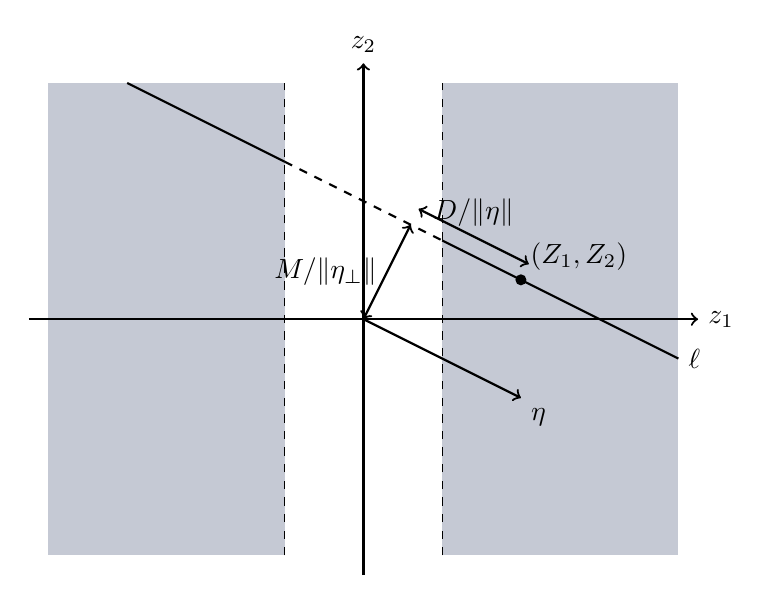
\begin{tikzpicture}
  \fill[l-color0] (-4, -3) -- (-4, 3) -- (-1, 3) -- (-1, -3) -- cycle;
  \fill[l-color0] (4, -3) -- (4, 3) -- (1, 3) -- (1, -3) -- cycle;
  \draw[thick, ->] (0, -3.25) -- (0, 3.25) node[above] {$z_2$};
  \draw[thick, ->] (-4.25, 0) -- (4.25, 0) node[right] {$z_1$};
  \draw[dashed] (-1, -3) -- (-1, 3);
  \draw[dashed] (1, -3) -- (1, 3);
  \fill (2, 0.5) circle(2pt) node[above right] {$(Z_1, Z_2)$};
  \draw[thick, ->] (0, 0) -- (2, -1) node[below right] {$\eta$};

  \draw[thick, <->] (0, 0) -- (0.6, 1.2) node[midway, left] {$M / \|\eta_\perp\|$};
  \draw[thick] (-3, 3) -- (-1, 2);
  \draw[thick, dashed] (-1, 2) -- (1, 1);
  \draw[thick] (1, 1) -- (4, -0.5) node[right] {$\ell$};

  \draw[thick, <->] (0.7, 1.4) -- (2.1, 0.7) node[midway, above] {$D / \|\eta\|$};
  \end{tikzpicture}
\end{frame}

\begin{frame}{Defining replicability}
  What do we estimate when we ``estimate replicability?''
  \vs
  {\bf RP:P statistic 3:} $83\%$ of the effect size estimates declined from original to replication
  \vs
  {\bf Definition 3:} Overall effect decline
  \begin{itemize}
  \item {\em What fraction of effect sizes declined by at least $20\%$?}
  \item Refers to {\em true} effect sizes, not point estimates
  \end{itemize}
  \vs
  Answers question: ``Do effects systematically attenuate in replications?'' 
\end{frame}

\begin{frame}{Defining replicability}

  {\bf Definition 3:} Overall effect decline
  \begin{center}
  	{\em What fraction of effect sizes declined by at least $20\%$?}
  \end{center}
  \vs
  Did replication $i$ show decline by at least $\rho \in [0,1]$?
  \[
  	H_i^{D,\rho}: S_i \cdot \theta_{i,R} \;\ge\; S_i \cdot (1-\rho) \theta_{i,O}
  \]
  % Oral: e.g. if rho = 20% and the original effect size was positive, the null hypothesis is theta_iR less than 0.8 times theta_iO$
  \vs
  After conditioning on $S_i$, this is a linear hypothesis in $(\theta_{i,R},\theta_{i,O})$
  \begin{itemize}
  	\item Use \citet{Lee:2016fv} test for individual $H_i^{D,\rho}$
  	\item Aggregate to estimate / bound fraction that declined by $\rho$
  \end{itemize}
\end{frame}


\section{Assessing replicability}

\begin{frame}{False directional claims}
  Work with adjusted $p$-values: conditionally, $p_{i,O} / 0.05 \gest U[0,1]$, under $H_i^{S,O}$
  \vs
  \begin{center}
  	\includegraphics[width=0.45\hsize]{fdp-original.pdf}
	\end{center}
  \vs
  {\bf NB:} no spike near 1 ($p_{i,O} \approx 0.05$)
\end{frame}

\begin{frame}{Inference on $\text{FDP}_{0.05}$}
  \begin{center}
  \begin{tabular}{lccc}
    \hline
    Adjusted $p$-value & $H_i^{S,O}$ true & $H_i^{S,O}$ false & Total \\
    \hline
    $20p_{i,O} \le \lambda$ & $*$ & $*$ & $*$ \\
    $20p_{i,O} > \lambda$ & $U$ & $*$ & $B$ \\
    Total & $V_{0.05}$ & $*$ & $R_{0.05} = m$ \\
    \hline
  \end{tabular}
  \end{center}
  \vs
  Inferences based on:
  \begin{equation}\label{eq:B}
    B \ge U \gest \text{Binom}(V, 1-\lambda)
  \end{equation}
  $\EE B \geq (1-\lambda)V_{0.05}$ leads to estimator \citep{Storey:2002vj}:
  \[
  	\widehat{\text{FDP}}_{0.05} = \frac{B}{R_{0.05}(1-\lambda)} = 2B/m \;\; \text{ if } \lambda = 1/2
  \]
  \vs
  \eqref{eq:B} also gives UCB $V_{0.05}^*$, leads to UCB 
  \[
  	\text{FDP}_{0.05}^{*} =  V_{0.05}^* / R_{0.05}
  \]
\end{frame}

\begin{frame}{Related questions}
  So far, asking about Type S error:
  \begin{itemize}
  	\item Does $S_i$ is correctly describe $\sgn(\theta_{i,O})$? (true orig.\ effect)
  \end{itemize}
  \vs
  Two related questions:
  \begin{itemize}
  	\item Does $S_i$ correctly predict $\sgn(\theta_{i,R})$? (true repl.\ effect)
  	\item Would Type S error be better if we'd used a different threshold, e.g.\ $0.005$?
  \end{itemize}
  \vs
  Requires slightly more subtle methods, similar in spirit  
\end{frame}

\begin{frame}{Results: False directional claims}
	Note:
	\begin{itemize}
		\item Estimate FDP $\approx 32\%$ for $0.05$ threshold
		\item For $\alpha = 0.005$, estimate is $7\%$, UCB $18\%$
		\item But not clear that FDP for replications is improved
		\item Numbers {\color{red} overestimate} Type S error ($\theta = 0.001$ similar to $0$).
	\end{itemize}
	\vs
	\centering
	Estimates / CIs for false directional claims
	\begin{tabular}{rr@{}lr@{}lrr}
	  \hline
	  $\alpha$ & Orig.\ Est. && Orig.\ U.C.B. && Repl.\ Est. & Repl.\ U.C.B. \\
	  \hline
	  $0.001$ & $2\%$& & $9\%$& & $27\%$ & $55\%$ \\
	  $0.005$ & $7\%$& & $18\%$& & $36\%$ & $61\%$ \\
	  $0.01$ & $11\%$& & $22\%$& & $39\%$ & $61\%$ \\
	  $0.05$ & $32\%$ && $47\%$ && $47\%$ & $63\%$ \\
	  \hline
	\end{tabular}
\end{frame}

\begin{frame}{Results: Effect shift}
  We construct $95\%$ CIs for $\theta_{i,O}-\theta_{i,R}$:
  \begin{itemize}
	  \item $15\%$ of studies exclude $0$ (exact replication), adjusting for selection
	  \item $39\%$ of studies rejected, otherwise
	  \item $11\%$ exclude $0$ after $\text{BH}_{0.1}$ correction, $1$ after Bonferroni
  \end{itemize}
\end{frame}

\begin{frame}{Results: Effect shift}
	\centering
	\includegraphics[width=0.75\hsize]{ci.pdf}
\end{frame}

\begin{frame}{Results: Effect decline}
  Estimate $35\%$ of effects declined by at least $20\%$
	\centering
	\includegraphics[width=0.8\hsize]{effect-decline-range.pdf}
\end{frame}

\begin{frame}{Takeaways}
  Selection bias is a powerful force
  \begin{itemize}
	  \item Leads to many predictable pathologies
	  \item Can't learn anything else without accounting for it
	  \item Truncated Gaussian model opens many avenues for inference
  \end{itemize}
  \vs
  Replicability has many possible meanings
  \begin{itemize}
  	\item Precisely specifying estimand is essential for meaningful discussions
  \end{itemize}
  \vs
  Rate of Type S errors in experimental psych is high: ($\approx 32\%$ of publ.?)
  \begin{itemize}
  	\item Reducing threshold to $0.005$ seems to improve FDP w.r.t.\ orig.\ effects
  	\item Doesn't mean results will be replicable in new experiments
  \end{itemize}
  \vs
  Evidence in a few studies that true effect sizes differ substantially
  \vs
  Some evidence of systematic effect decline (need more data)
\end{frame}

\begin{frame}{Future work}
\begin{itemize}
	\item Preregistration
	\begin{itemize}
		\item Better publication bias model
		\item Less conservative estimate: information of nonsignificant studies are useful still!
	\end{itemize}
	\item Higher powered design, e.g.\ \citet{Camerer:2018de,Klein:2018}
  \item More formal criteria
  \item Clearer picture of the replicability crisis
\end{itemize}
\end{frame}

\begin{frame}
\centering
{\Large Thanks!}
\end{frame}

\begin{frame}[allowframebreaks]{References}
\footnotesize{
\bibliography{papers,additional}
\bibliographystyle{plainnat}
}
\end{frame}

\end{document}